% \documentclass[preprint]{kcc}
\documentclass{kcc}


%%%%%%%%%%%%%%%%%%%%%%%%%%%%%%%%%%%%%%%%%%%%%%%
% include additional packages you need to use
%%%%%%%%%%%%%%%%%%%%%%%%%%%%%%%%%%%%%%%%%%%%%%%
% graphic, float package
\usepackage{graphicx}   % for setting images
\usepackage{float}      % for float objects
\usepackage{subfigure}  % for adding several figures in a figure environment
\usepackage{lscape}     % for landscape type images or tables

% Reduce the line spacing in the bibliography
\let\oldbibliography\thebibliography
\renewcommand{\thebibliography}[1]{%
  \oldbibliography{#1}%
  \setlength{\itemsep}{0pt}%
}

\usepackage{enumitem}

% for compact section title spacing
% \usepackage[compact]{titlesec}

% nameref
\usepackage{nameref}

% mathmetical presentation
\usepackage{gensymb}
\usepackage{amsmath}
\usepackage{dsfont}
\usepackage{amssymb}
\usepackage{amsthm}
\usepackage{exscale}
\usepackage{textcomp}   % extra symbols


% for circled number
\newcommand{\cl}[1]{\textcircled{\scriptsize #1}}


% package for using algorithmic presentation
\usepackage{algorithmic}
\usepackage{algorithm}
% customize algorithmic environment
\renewcommand{\algorithmicrequire}{\makebox[40px]{\hfill\textbf{Input :}}}
\renewcommand{\algorithmicensure}{\makebox[40px]{\hfill\textbf{Output :}}}

\DeclareMathOperator*{\argmin}{\arg\!\min}
\DeclareMathOperator*{\argmax}{\arg\!\max}

% array and table presentation
\usepackage{array}
\usepackage{tabulary}
\usepackage{multirow}
\usepackage[table]{xcolor}
\usepackage{ctable}
\usepackage{booktabs}   % for typesetting tables at the level of publication
                        % do not use vertical rule
\usepackage{lipsum}
              
% set title, author, abstract
\title{시선 정보를 이용한 만화 영상의 가속화된 선택적 학습 방법}
\author{
김진화$^{\circ1}$, 장병탁$^{12}$\\
서울대학교 인지과학 협동과정$^{1}$\\
서울대학교 컴퓨터공학부$^{2}$\\
\{jhkim, btzhang\}@bi.snu.ac.kr
}
\engtitle{Accelerated Selective Learning from Cartoon Videos with Eye-Gaze Information}
\engauthor{
}
\abstract{
이미지-텍스트 다중 모달(multimodal) 학습에 대한 많은 선행 연구에서 입력 이미지에 대응하는 문자열을 생성하기 위한 다양한 모델을 제안하였다. 본 연구에서는 콘볼루션(convolution) 시각 특징 벡터를 선택적으로 순환 학습하는 조건화 LSTM(Conditional Long Short-Term Memory)과 LRCN(Long-term Recurrent Convolutional Networks) 모델을 결합하여 학습하는 모델을 제안한다. 여기서 문자열을 구성하고 있는 한 단어는 주어진 이미지의 일부 영역과 대응될 수 있다는 가정을 전제한다. 본 연구에서는 만화 영상과 같이 입력 이미지들이 시간 축 상에서 문맥적 흐름을 가질 때 한 단어와 이미지의 한 영역의 대응 관계는 문맥에 따라 달라질 수 있다는 가정으로 조건을 완화하여 선행 연구를 확장한다. 문맥 기반 주의 모델을 학습하기 위하여 선행 학습으로 한 시간 분량의 비슷하지만 다른 영상 정보에 대하여 수집 된 다수 사람들의 시선 분포 정보를 이용함으로써 선택적 학습을 가속화 한다.
}

\begin{document}

\maketitle


\section{서 론}

다중 모달 학습은 서로 다른 통계적 성질을 가진 모달 간의 공통된 정보를 학습한다. 그러나 이러한 각 모달의 통계적 차이가 입력된 데이터에 대하여 직접적인 공통된 정보를 얻기 어렵게 만든다. 따라서 많은 선행연구에서는 깊은 학습(deep learning)을 통해 각 모달의 상위 개념을 먼저 학습한 후 공통된 정보를 학습하는 방법을 이용하였다\cite{Ngiam2011,NIPS2012_4683,Kiros2013,NIPS2014_5279}. 이미지-텍스트 다중 모달 학습에서 이미지에 포함된 여러 독립적인 객체들과 자연어 언어 모델 안에서 단어와의 관계를 문법적 정보나 예제 문장 틀과 같은 선행 지식 없이 자동적으로 학습하는 연구에서 성능적으로 많은 진보가 있었다\cite{Kiros2013,Yu2013,Karpathy}.

Xu et al.\cite{Xu2015}의 연구에서는 이미지 안의 여러 독립 객체들과 문장과의 관계를 자연어 언어 모델 안에서 동적으로 학습하는 모델을 제안하였다. 자연어 언어 모델 학습에 좋은 성능 보이고 있는 순환 네트워크의 일종인 LSTM 모델에서 은닉 상태에 따라 주어진 이미지의 콘볼루션(convolution) 시각 특징 벡터 일부를 공간 상에서 선택, 순환 학습함으로써 주의 모델 기반 조건화 LSTM을 구현하였다. 변분 베이지안(variational Bayesian) 방법에서 변분 최소 경계(variational lower bound)를 최대화하는 새로운 목적 함수를 정의하고, 이 새로운 목적 함수에 적용 가능한 몬테 카를로(Monte Carlo) 샘플링을 이용하여 비용 함수의 경사도를 계산하기 때문에 일반적인 역전파(back-propagation) 알고리즘을 통해 LSTM과 신경망 네트워크인 주의 모델을 일관된 방법으로 두 모듈을 동시에 학습할 수 있다.

하지만 기존 연구는 정적 이미지에 대한 기술적 문장을 생성하도록 학습하기 때문에, 만화 영상과 같이 시간의 흐름에 따라 문맥이 달라질 수 있는 데이터에는 적합하지 않다. 예를 들면 동일한 두 캐릭터가 대화를 나누는 같은 장면도 앞에서 무슨 행동이나 대화를 나누었냐에 따라 문맥이 달라지며 해당 장면에 대한 대사가 달라질 것이다. 따라서 우리는 기술적으로 기존 연구에서 두 가지 요소를 변경하여 문제를 해결하고자 한다. 첫 번째는 LSTM의 메모리 벡터 $c_0$와 은닉 벡터 $h_0$를 새로운 이미지에 따라 초기화 하지 않고 보존한다. 두 번째는 주의 모델 $f_{att}$를 랜덤 파라미터로 초기화하는 대신 한 시간 분량의 비슷하지만 서로 다른 영상을 본 다수 사람들의 시선 분포 정보를 이용하여 파라미터 값을 초기화 함으로써 선택적 학습을 가속화 하고자 한다.  

따라서 본 연구는 입력 이미지들이 시간 축 상에서 문맥적 흐름을 가질 때 한 단어와 이미지의 한 영역의 대응 관계는 문맥에 따라 달라질 수 있다는 가정으로 선행 연구를 확장한다. 이 때 입력 이미지 내 독립 객체들의 상호 작용이 문맥 조건에 따라 달라지고 문장 내의 단어들과의 상호 작용도 더욱 동적으로 일어난다. 

\section{Attentional LSTM}

LSTM 모델은 입력 벡터의 일부가 출력되는 재귀적인 구조를 가진다. $t-1$ 시간에서의 출력 벡터 $y_{t-1} \in \mathbb{R}^K$의 선형 사영값 $Ey_{t-1} \in \mathbb{R}^m$와 은닉 벡터 $h_{t-1} \in \mathbb{R}^n$, 그리고 $t$ 시간에서의 문맥 벡터 $\hat{z}_t \in \mathbb{R}^D$를 입력하면 $t$ 시간에서의 은닉 벡터 $h_t$를 출력한다. 여기에서 $y$는 단어를 나타내는 비트 지시 벡터(해당 단어 인덱스가 1이고 나머지는 0인 벡터)이고 $h$는 LSTM의 학습 파라미터 벡터, $\hat{z}$은 주의 모델 $f_{att}$의 출력 값이다. LSTM 모델에서 정규화 방법을 제안한 Zaremba et al.\cite{Zaremba2015}의 방법에 따라 LSTM을 구현하면 다음과 같이 표현할 수 있다.

\begin{equation}
\begin{pmatrix}i_{t}\\f_{t}\\o_{t}\\g_{t}\end{pmatrix} =
  \begin{pmatrix}\mathrm{\sigma}\\\mathrm{\sigma}\\\mathrm{\sigma}\\\tanh\end{pmatrix}
  T
  \begin{pmatrix}Ey_{t-1}\\h_{t-1}\\\hat{z}_t\end{pmatrix}
\end{equation}

\begin{equation}
c_t = f_t \odot c_{t-1} + i_t \odot g_t\\
\end{equation}
\begin{equation}
\label{eq3}
h_t = o_t \odot \tanh(c_t)\\
\end{equation}

$E \in \mathbb{R}^{m \times K}$는 단어를 나타내는 비트 지시 벡터를 실수값으로 선형 사영한다.  $T \in \mathbb{R}^{D+m+n \times n}$는 LSTM의 내부 파라미터 행렬이다. $E$와 $T$는 연쇄 법칙에 따라 목적 함수에 의해 역전파 알고리즘으로 학습되는 파라미터 행렬이다. 수식\ref{eq3}에 따라 $h_t$를 구한다면 다음 식을 이용하여 $y_t$를 구할 수 있게 된다.

\begin{equation}
p(y_t|y^{t-1}_1,a) \propto \exp{L_o(Ey_{t-1} + L_{h}h_t + L_{z}\hat{z}_t))}
\end{equation}

여기에서 $L_{o} \in \mathbb{R}^{K \times m}$, $L_{h} \in \mathbb{R}^{m \times n}$, $L_{z} \in \mathbb{R}^{m \times D}$는 모두 목적 함수에 의해 학습되는 파라미터 행렬이다.

\begin{figure*}
  \centerline{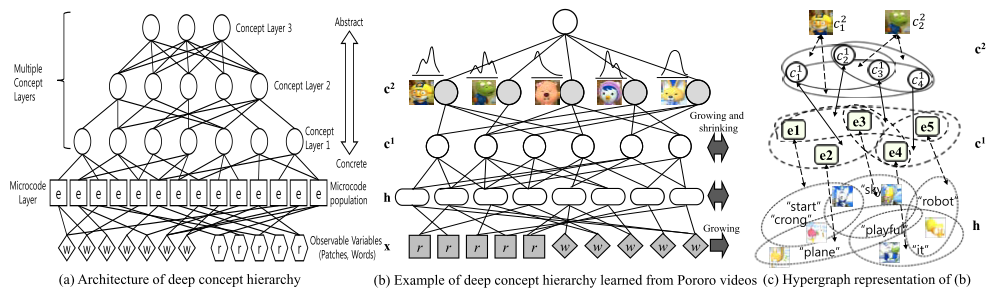
\includegraphics[width=180mm,height=54mm]{eps/ha2015_fig2.png}}
  \caption{DCH 모델의 이론적 개념도. (a)는 DCH의 계층 구조를 보여주며, (b)는 두 개의 개념 계층 망을 가지고 뽀로로 만화 영상에 대한 개념도를, (c)는 (b)에 대한 하이퍼그래프 표상을 나타낸다. (b)에서 c2는 지도 학습 목표가 되는 캐릭터 등장 라벨을, r과 w은 데이터에서 관찰된 값을 나타내며, r은 이미지 특징 벡터에 대한 노드를, w는 자막 텍스트에 대한 노드를 나타낸다. 모델에 대한 이해를 돕기 위해 저자의 동의를 얻어 본 논문에 포함하였다 \cite{Ha2015}.}
  \label{fig:ha2015}
\end{figure*}



\begin{equation} 
\begin{split}
G^{*} & = \argmax_{G_{t}} P(G_{t}|D) \\
      & = \argmax_{G_{t}} P(D|G_{t})P(G_{t-1}) \\
\end{split}
\end{equation}

이 모델은 각 영상 이미지에 등장하는 캐릭터를 나타내는 지표 벡터 $y \in \mathds{R}^{|c2|}$를 이용하여 지도 학습을 하게 된다. 형식적으로 아래와 같이 관찰된 데이터와 캐릭터 지표 벡터를 통해 하이퍼그래프를 구성한다.

\begin{equation}
\begin{split}
P(G|D,y) & = \frac{P(D|G,y) P(y|G) P_{t-1}(G)} {P(D,y)} \\
\end{split}
\end{equation}

여기서 $P(D|G,y)$는 데이터 재생성 항으로서 모든 하이퍼엣지의 학습된 가중치의 합 대비 데이터에 대하여 연결된 하이퍼엣지 가중치 합의 비율로 정의 되며 softmax 함수, 또는 다른 표현으로, 정규화된 지수 방법을 사용한다. 가중치는 전적으로 관찰(샘플링) 된 데이터의 빈도 수에 따라서만 조정되므로 그래프 몬테 카를로 방법에 따라서 그 성능이 크게 변하게 되며 의존적 이다\cite{zhang1994accelerated,Zhang1998}. 자세한 내용은 하정우 등\cite{Ha2015}의 논문을 참고하길 바란다.

\section{Hybrid 그래프 몬테 카를로}
위의 모델에서 가장 효과적인 그래프 몬테 카를로 방법으로 보상적 그래프 몬테 카를로(FGMC) 방법을 제안 하였다. 이 샘플링 기법은 샘플링이 적게 된 노드를 더 많이 샘플링 되도록 한다. 따라서 시각-언어 번역 테스트에서 정확도는 다른 기법에 비해 소폭 상승하였지만 재현도에서 상대적으로 큰 값을 가졌다. 빈도 수가 상대적으로 작은 특징들에 대해 보다 정확한 경험적 확률 분포를 얻기 위한 방법으로 크고 희소한 그래프를 만들게 됨으로써 비효율적 그래프를 학습하게 된다.

이러한 원인은 그래프 몬테 카를로 방법에 의한 가중치 조정이 추론의 중요한 요인이 됨에도 불구하고 언어 정보를 직접적으로 추론할 수 없는 낮은 수준의 특징 값인 SIFT 특징 벡터들을 샘플링 대상으로 삼기 때문에 효율적인 샘플링을 위한 정보가 부족하다. 본 연구에서는 이러한 언어 정보를 추론하는 데에 도움을 줄 수 있는 1시간 분량의 영상에 대한 다수 사람의 시선 분포 정보를 이용하여 SIFT 특징 벡터들을 샘플링 하는 방법을 제안하고자 한다.

다수 사람의 시선 분포 정보는 모든 데이터 입력에 대한 값을 실험적으로 가지는 것은 비효율적이므로 컨볼루션 신경망(Convolutional Neural Networks)을 이용하여 입력 이미지 $\mathcal{I}$에 대한 분포 추정 값 $\hat{\pi}$을 관찰된 시선 분포 $\pi$를 통해 얻는다. 여기서 컨볼루션 신경망의 마지막 층은 분포에 대한 오차를 에러 함수로 정의한 후 파라미터 값들을 어렵지 않게 학습할 수 있다. $\hat{\pi}$를 이용한 아래의 수식은 기존 연구의 그래프 몬테 카를로 방법으로 치환하게 된다.

\begin{equation} 
\begin{split}
P(v_{i}) & = \frac{\exp(\hat{\pi}(pos(v_{i})) \cdot w_{i} \cdot log(R(d(v_{i}))))}{Z}
\end{split}
\end{equation}

수식~\ref{eq3}에서 함수 $pos(v_{i})$는 노드 $v_{i}$의 이미지 $\mathcal{I}$ 상에서의 위치를, 함수 $d(v_{i})$는 학습된 하이퍼그래프 안에서 연결된 정도(degree), 함수 $R$은 가능한 집합 내 $v_{i}$의 순위를 나타낸다. 순위 값은 로그 크기 조정 후 사용한다. $w_{i}$은 현재 관찰된 빈도 수를 나타낸다. 이미지 $\mathcal{I}$에서 추출한 SIFT 특징 벡터는 클러스터링을 통해 한 노드로 표현되므로 빈도 수가 1 이상일 수 있다. 수식~\ref{eq4}는 총 합이 1이 되게 하는 분모를 나타낸다.

\begin{equation} \label{eq4}
\begin{split}
Z & = \exp(\sum_{i=1}^{|v|}{P(v_{i})})
\end{split}
\end{equation}

\begin{figure}
  \centerline{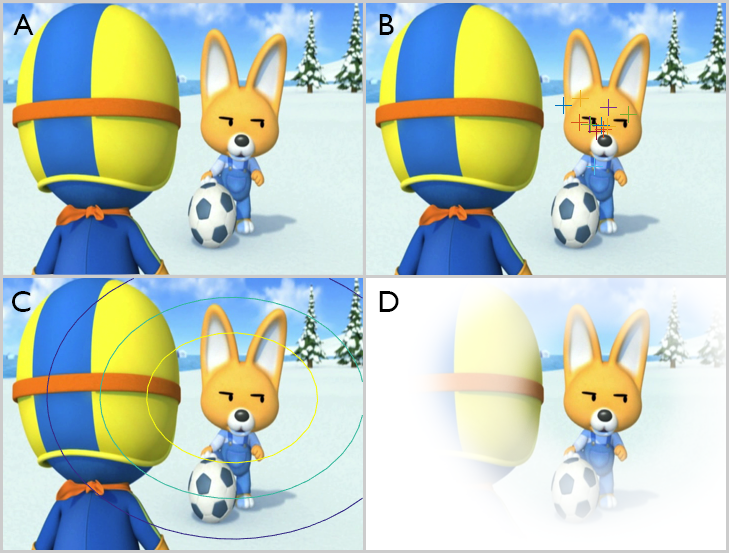
\includegraphics[width=92mm,height=70mm]{eps/sel_fig2.png}}
  \caption{시선 정보를 활용하는 방법을 도식화. A는 원본 이미지, B는 만화 영화 시청 상황에서 A의 이미지에 해당하는 프레임 시각에 응시한 서로 다른 13명의 응시 좌표들을 십자가 기호로 나타내었다. C는 응시 좌표들을 가우시안 혼합 모델(Gaussian Mixture Model)로 나타냈을 때의 확률 분포를 세 개의 등고선으로 어림 표현하였다. D는 그래프 몬테 카를로 방법으로 샘플링할 SIFT 벡터의 확률 가중치를 도식적으로 표현한다. 컨볼루션 네트워크에서 학습할 분포는 C의 분포가 된다.}
  \label{fig:selective}
\end{figure}

\iffalse
\begin{figure}
  \centerline{\includegraphics[width=60mm,height=54mm,trim=65mm 103mm 68mm 100mm]{}}
  \caption{긴 응시와 짧은 응시에 대한 장기 기억 능력 시험 결과 이다. 긴 응시와 짧은 응시에 대한 기억력 점수는 통계적으로 유의미 하지 않았다(p $=$ 0.5051). 오차 막대는 $\pm$ 2 표준 오차를 뜻 한다. 실험에 대한 자세한 설명은 ~\nameref{subsec:experiment2} 소절을 참조한다.}
  \label{fig:memtest-leng}
\end{figure}

\begin{figure}
  \centerline{\includegraphics[width=60mm,height=54mm,trim=55mm 108mm 58mm 105mm]{}}
  \caption{}
  \label{fig:memtest-nested}
\end{figure}
\fi

\section{토 론}

그래프 몬테 카를로를 영상 데이터에 사용하게 된 것은 풀고자 하는 문제가 정확한 객체 인식의 문제에서 정확한 개념 형성의 문제로 치환되었기 때문이다. 객체 인식의 문제에서는 모델 학습이 풀고자 하는 분류의 범위가 고정되고 입력 데이터의 범위도 그 분류 범위 안에 존재한다는 특수한 강한 가정을 하고 있기 때문에 그 성능을 보장하는 대신 응용 범위를 제한한다. 반면, 영상 데이터를 이용한 시각-언어 개념 학습 모델에서는 분류의 범위와 데이터의 범위가 이론적으로 무한하다. 이러한 조건에서 전반적인 성능 하락을 경험하지 않기 위해서는 파라미터 수 역시 늘어나지 않을 수 없으며, 결국 유연한 모델과 학습 방법을 요구한다 \cite{zhang1994incremental}. 그래프 몬테 카를로 방법은 간단히 관찰 빈도 수 기반으로 네트워크 모델을 학습하지만 다른 영역의 학습 모델과의 접점을 제공한다.

본 연구에서는 그래프 몬테 카를로 방법에서 메타 정보라고 할 수 있는 관찰된 사람의 시선 정보를 이용한다. 다수 사람들의 시선 정보를 분포로 얻은 후 컨볼루션 네트워크로 그 분포를 학습하고 새로운 입력 데이터에 대해서 재생성 할 수 있기 때문에 유용하다. 사람의 시선 정보는 시각 자극에 의존적인 상향식 주의와 시계열에 따른 문맥 등을 고려한 전전두엽의 고차원적인 선택적 주의인 하향식 주의가 합성되어 있지만 본 연구에서는 다수 시선 정보 분포로 변환 후 단일 입력 이미지에 대한 분포를 학습함으로 상향식 주의 모델을 만들게 된다. 시계열 정보를 이용한 하향식 주의 모델을 고려할 수 있겠지만 컨볼루션 네트워크가 아닌 순환 네트워크 모델이 필요하고 그에 따른 모델의 복잡도 대비 성능 개선의 정도가 불투명하기 때문에 본 연구에서는 고려되지 않았다.

\section{결 론}

영상 정보와 같이 서로 다른 양태들의 표상들의 관계를 학습할 할 때에는 효과적인 학습 알고리즘이 필요하다. 기존 연구에서는 하이퍼그래프와 그래프 몬테 카를로 방법을 이용하여 희소하지만 효과적인 방법을 제안하였다. 그러나 FGMC 방법은 비효율적인 모델을 유도하므로 한계를 지니고 있다. 본 논문에서는 메타 정보인 사람의 시선 분포 정보를 컨볼루션 네트워크로 학습한 뒤 그래프 몬테 카를로 방법에 적용하는 혼용법을 제안한다. 컨볼루션 네트워크로 학습된 상향식 주의 모델은 관찰된 데이터에서 탐색 공간을 효과적으로 줄이게 된다. 

\section{감사의 글}
이 논문은 2015년도 정부(미래창조과학부)의 재원으로 한국연구재단의 지원(NRF-2010-0017734-Videome)과 정보통신기술진흥센터의 지원(R0126-15-1072-SW스타랩, 10035348-mLife, 10044009-HRI.MESSI)을 받아 수행된 연구임.

\bibliographystyle{ieeetr}
\bibliography{KidsVideo-selective}

\end{document}
